\section{Architecture}

\subsection{Hardware Choices}

Using the LEGO NXT was a given from the project start, which means we will also be using two LEGO Mindstorms
motors as actuators for turning the turret. The firing will be done using the LEGO Technic competition cannon
using an additional motor to pull the trigger. Additionally, we use two LEGO Minstorms touch sensors to ensure
a correct reset of the tower.

For detection, the Microsoft Kinect was chosen over the LEGO Sensors. The primary reason for this is that
it enables three-dimensional detection with a single piece of hardware, as opposed to the LEGO sensors where
an Ultrasound will only detect distance, and a different sensor would be needed for the remaining two dimensions.
Additionally, using image analysis allows for a wider range of targets, as an algorithm can be tweaked to
fir the target, but the limitations on the surfaces an ultrasound sensor can detect are determined by the
hardware itself.

Using the Kinect Camera does require a PC acting as a proxy between the camera and the NXT, or modding the
NXT itself to allow for the connections. For ease of implementation, and because the group did not own the NXT
used in the project, a PC was used over hardware modding. This PC is connected to the NXT using USB.
Thus, the architecture ends up like seen on \autoref{fig:archictecture1}

\begin{figure}[hbtp]
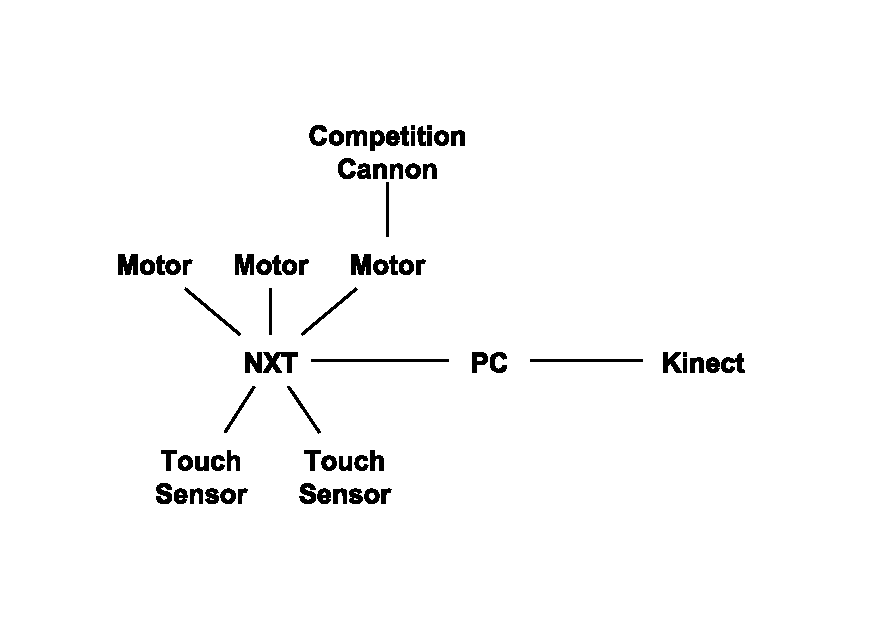
\includegraphics[width=0.75\textwidth]{img/architecture1.pdf}
\caption{Architecture Diagram} 
\label{fig:archictecture1} 
\end{figure}

\subsection{Software Choices}